\section{Hardware}
\label{sec:chapterexample}

Das System wird Hardwareseitig in zwei Teile unterteilt. Der Server, die zentrale Einheit und die Aussensprechstelle.
\\
\\
Die \cref{tbl:SrvHW} und die \cref{tbl:DoorHW} zeigen die benötigten HW-Komponenten, welchen an die jeweilige Stellen benötigt werden.
\\
Um den Überblick über die Kosten aller Hardware-Komponenten zu behalten, sind hier auch die Preisen aufgelistet. Wichtig hier ist sicherzustellen, dass die gesamten Hardwarekosten diejenigen der von der Konkurrenz angebotenen Produkte nicht übersteigen.
\\
Die Preise können natürlich leicht abweichen da es sich um Standardkomponenten handelt und die Preise sich schnell ändern. Die Summen sind mehr als Kostenschätzung zu betrachten.

\begin{table}[]
	\centering
	\label{my-label}
	\begin{tabular}{l|ll}
		\multicolumn{1}{r|}{} \textbf{Anzahl} & \textbf{Komponent} \hspace{180pt} & \textbf{Preis} 	\\ \hline
		1	&	Raspberry Pi 3 Model B						& 50.-				\\ \hline
		1	&	Raspberry Gehäuse und Netzteil				& 25.-			\\ \hline
		2	&	8-Kanal Relais Modul						& 15.-			\\ \hline
		1	&	\textit{Kleinmaterial}						& 15.-			\\ \hline
		\textbf{Total}	&									& \textbf{140.-}			\\ \hline
	\end{tabular}
	\caption{Server HW Komponenten}
	\label{tbl:SrvHW}
\end{table}

\begin{table}[]
	\centering
	\label{my-label}
	\begin{tabular}{l|ll}
		\multicolumn{1}{r|}{} \textbf{Anzahl} & \textbf{Komponent} \hspace{180pt} & \textbf{Preis} 	\\ \hline
		1	&	Raspberry Pi 3 Model B		   				& 50.-			\\ \hline
		1	&	4" Bildschirm								& 64.-			\\ \hline
		1	&	Raspberry Kamera							& 59.-			\\ \hline
		1	&	PoE Adapter									& 50.-			\\ \hline
		3	&	Schalter									& 25.-			\\ \hline
		1	&	Mikrophon									& 12.-			\\ \hline
		1	&	Lautsprecher								& 9.-			\\ \hline
		1	&	Audio Verstärker							& 10.-			\\ \hline
		1	&	\textit{Kleinmaterial / Gehäuse}			& 50.-			\\ \hline
		\textbf{Total}	&									& \textbf{329.-}			\\ \hline
	\end{tabular}
	\caption{Aussensprechstelle HW Komponenten}
	\label{tbl:DoorHW}
\end{table}


\subsection{Server}
\label{sec:chapterexample}

Der Server wird mit einem Relay-Board verbunden. Diese wird die Gongs und die Türöffner bedienen. An dieser Stelle ist die Hardware-Konfiguration sehr einfach. Je nach wie viele Gongs und Türe verbunden werden müssen, könnten bis zwei 8-Channel Relayboards verbunden werden.
\\

<-- ABBILDUNG CON LA PI E I RELAY E I PIN A CUI SONO COLLEGATI
\\
\\

\subsection{Aussensprechstelle}
\label{sec:chapterexample}

Bei der Aussensprechstelle wird auch eine Raspberry Pi eingesetzt. Hier sind mehrere Zusatzkomponenten notwendig. Die Speisung an dieser stelle erfolgt nur über PoE, aus diesem Grund ist PoE-Splitter vorhanden.
\\
\\
Für die Audiowiedergabe ist ein kleines Lautsprecher und ein Verstärker nötig. Die Chinch-Anschluss der Raspberry Pi hat eine zu kleine innere Widerstand um direkt ein solches Lautsprecher anschliessen zu können. Die Hauptproblematik nun besteht darin, dass die Massen des Raspberry Pi, der Verstärker und des Audio-Interface alle zusammen gekoppelt sind. Das führt zu Brunschleifen die wiederum Störsignale auf dem Audio-Ausgang erzeugen. Um das zu vermeiden ist eine Massentrennfilter an dieser Stelle notwendig.
\\

<-- ABBILDUNG CON LA PI E COMPONENTI COLLEGATI
\\
\\

\subsection{Microcontroller Problematik}
\label{sec:microcontroller}
WebRTC basiert, für den Video encoding auf den von Google Inc. offengelegte VP8 codec. Der Codierung im Gegensatz zu den Decodierung, wie bei der Mehrheit solche Systemen ist sehr Leistungsintensiv. Die Situation kommt bei der Aussensprechstelle genau so vor, dort wird der Videostream auf den Raspberry Codiert und am Server für die Decodierung weitergeleitet. Diese bringt, was der Rechenkapazität anbelanget,  die Rapspberry  an ihre Grenzen. Die Problematik stellt für End-Qualität des Streaming eindeutig den Flaschenhals dar. Obwohl eine Kamera mit hohe Auflösung im Einsatz ist, wird WebRTC anhand des niedrige Framerate die Qualität des Stream verringern. Sobald die Qualität herabgestzt ist, ist die Raspberry im Stand die Codierung im Echtzeit durchzuführen.
\\
Aufgrund der hohe überlastung des Prozessor, die während der Kodierung unterworfen ist, zeigen sich Wärmeabführung Probeme. Bei einer verlängerte Videostreaming Session, was normalerweise bein eine Türsprechanlage nicht der Fall ist, könnte der Raspberry zu einer Absturz bringen. 
\\
Der Raspberry Pi 3 war während der Entwicklungsphase des Prototyp die richtige Entscheidung. Haptgrund war der hohe Kompatibilität, die Standardisierung bei ein soches sehr gut etabliertes Produktund und die Stabilität. Dazu kommen noch die Unzählige Infos, Dokumentationen die im Interet über diese Microcontroller zu finden sind.

\subsubsection{Alternative}
Mit den gesammelte Erfahrungen während der Prototyp Entwicklung kann eine bessere Alternative zur Raspberry für eine Weiterenwicklung der Anlage ausgewertet werden. 
\\
Der Microcontroller Banana Pi M3 hat in Gegensatz zum Raspberry erheblich mehr Datenverarbeitungsleistung zu bieten (\seeref{tbl:Comaparison}). Dazu kommt noch dass diese Microcontroller das H.264 hardware acceleration unterstüzt und somit der Videostream weiterhin optimisiert würde.

\begin{table}[]     
	\centering
	\label{my-label}
	\begin{tabular}{l|ll}
		\multicolumn{1}{r|}{} & Raspberry Pi Model 3 & Banana Pi M3 \\ \hline
		CPU Cores             & 4                    & 8            \\ \hline
		CPU Design            & Cortex A53           & Cortex A7    \\ \hline
		CPU Frequenz          & 1.2GHz               & 1.8GHz       \\ \hline
		Memory                & 1GB DDR2             & 2GB DDR3     \\ \hline
		Memory Frequenz       & 400MHz               & 672MHz       \\ \hline
		H264 Decoding         & 1080P30              & 1080P60      \\ \hline
		H264 Encoding         & 1080P30              & 1080P60      \\ \hline
		Preis				  & CHF 50.0             & CHF 99.00    \\ \hline
	\end{tabular}
\caption{Verwendete Raspberry Pi im Vegleich mit die Banana Pi Alternative}
\label{tbl:microcontrollerComparison}
\end{table}

Ein weiteres Vorteil des Banana Pi is das der Raspbian OS ebenfalls ünterstützt wird. Die mit dem Projekt mitgeliferte Image des Betriebsistem für die Aussensprechstellen könnte somit auf den neue Microcontroller mit geringere Aufwand aufgespielt werden. Auch die Verkabelung stellt kein Problem dar, da die Pinbelegung eins zu eins die von der Raspberri entspricht.

\subsection{PoE}
\label{sec:poe}
Moderne Hausalte werden meistens mit ethernet Verkabelung verlegt. Ziel des Aussensprechstelle ist die Installationskosten zu senken und die Montage zu vereinfachen. Drei Anschlusse werden von den Aussensprechstelle benötigt um sein Ziel zu erreichen und zwar Strom, Internetverbindung und eine Leitung der den Türöffner betätigt. Alle diese Fünktionalität können in einem Kat 7 Ethernet Kabel zusammengeführt werden. 
\\
Cisco Catalyst 3560g welcher für den PoE Stromversorgung zuständigt ist verwendet das Phantomspeisung oder Mode A. Das heisst dass die mit Datenübertragung belegten Adern mit der Stromversorgung überlagert werden. Diese ist möglich da Elektrizität eine niedrige Frequenz von 60 Hz hat und Datenübertragungen im bereich 10-100MHz liegen.

\begin{figure}[htb!]
	\begin{center}
		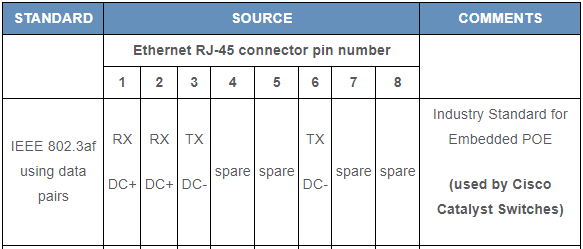
\includegraphics[width=0.89\textwidth]{CatalystPoEpinouts}
		\caption[Catalyst Pinouts]{Catalyst 3560g PoE Pinbelegung}
		\label{fig:catalystPinouts}
	\end{center}
\end{figure}

Wie im Abbild nr.5!!? dargestellt werden die Adern 7 und 8 dazu verwendet um der Türöffner zu betätigen. Aus den 3 verbliebenden Adernpaare kann maximal die Ethernet Kategorie 100BASE-T erreicht werden. Da aber WebRTC eine erhebliche kleinere Bandbreite in Anspruch nimmt, stellt für die Aussensprechtellen kein Hinderniss dar.

\begin{figure}[htb!]
	\begin{center}
		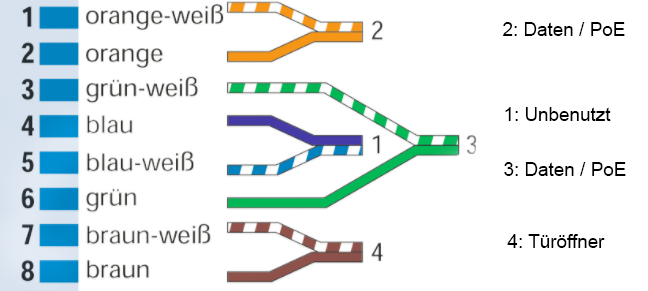
\includegraphics[width=0.89\textwidth]{EthernetPinbelegung}
		\caption[EthernetPinbelegung]{Cat. 7 Ethernet Pinbelegung für die Aussensprechstellen}
		\label{fig:catalystPinouts}
	\end{center}
\end{figure}


\newpage